\chapter{Evaluación}
\noindent
En este capítulo se mostrarán los datos sobre las evaluaciones escritas por usuarios que han probado la aplicación. Se ha evaluado el rol del deportista mediante una encuesta condicionada según las funciones probadas por el propio usuario.

\section{Diseño de la evaluación}
Para realizar esta evaluación se ha ofrecido un fichero ejecutable (APK) a un conjunto de personas para probar la aplicación. Se ha ofrecido esta aplicación a un total de 23 personas, mayormente jóvenes, algunos que ya tenían experiencia con todo lo relacionado con la nutrición, dado que lo hacían ya de manera habitual en su vida cotidiana y otros que no tenían la misma experiencia en nutrición y por tanto era más probable que optasen por seguir una dieta. 

La evaluación del usuario se ha realizado mediante un formulario de Google Forms \cite{googleForm} recogiendo, en varias secciones, los diferentes contenidos de la aplicación:

\begin{itemize}
    \item Una primera sección con las diferentes preguntas personales y características generales de la aplicación, es decir, funciones que todo el mundo ha pasado por ellas como el registro, el menú principal y su perfil. Al final de esa sección se realizará una pregunta sobre la sección de creación de una dieta en la cual en caso afirmativo saltará a la sección correspondiente realizando las diferentes preguntas sobre la creación y gestión de la dieta. En caso negativo saltará a un bloque común que realizará también el otro usuario una vez termine la sección de creación de la dieta.
    \item El bloque de la gestión de la dieta se encarga de realizar las preguntas respectivas a todo el tema de creación de la dieta, inserción de alimentos y modificación de la misma. Una vez finalizado se realizará una pregunta (tanto si contestaste que sí como si comentaste que no en la pregunta que saltó a este bloque) se realizará una pregunta en la que se cuestionara si el usuario ha seguido alguna dieta en su transcurso por la aplicación. Esta respuesta, en caso de ser afirmativa te redirigirá a otra sección con preguntas respectivas a dicho módulo y en caso negativo te redirigirá a la sección final de la encuesta.
    \item El tercer bloque de seguimiento de la dieta hace referencia, a la parte del menú principal de ``mi dieta`` con preguntas sobre la inserción de alimentos consumidos y de comentarios principalmente. Una vez finalizada saltará a la sección final donde se dará una nota al proyecto.
    \item El último módulo de la encuesta se basa principalmente en una valoración general de la dieta.
\end{itemize}

%%%%%%%%%%%%%%%%%%%%%%%%%%%%%%

\section{Resultados de la evaluación}
En la figura \ref{fig:grafico_1} se puede contemplar que casi un 62\% de los usuarios son del género masculino frente a un 38\% son del género femenino. Esto se debe a que la mayoría de los usuarios que resultan haber probado la aplicación son de la misma facultad.

\begin{figure}[H]
    \centering
    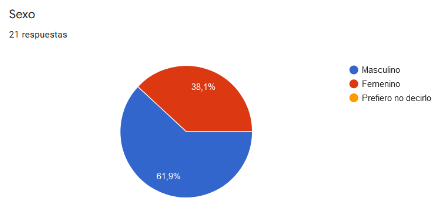
\includegraphics[width=0.9\textwidth]{Images/Capitulo8/Capitulo8.2/grafico1.png}
    \caption{Resultado de la pregunta de género}
    \label{fig:grafico_1}
\end{figure}

%%%%%%%%%%%%%%%%%%%%%%%%%%%%%%%%%
En la figura \ref{fig:grafico_2} se puede deducir que ningún usuario tuvo ningún problema a la hora de registrarse.

\begin{figure}[H]
    \centering
    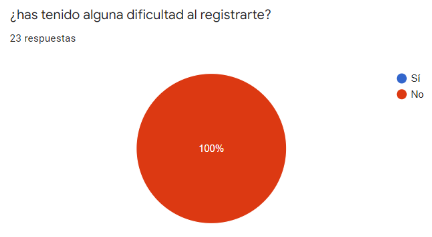
\includegraphics[width=0.9\textwidth]{Images/Capitulo8/Capitulo8.2/grafico2.png}
    \caption{Resultado de la pregunta de la dificultad de registro}
    \label{fig:grafico_2}
\end{figure}

%%%%%%%%%%%%%%%%%%%%%%%%%%%%%%%%%%%

En la figura \ref{fig:grafico_3} se puede observar que casi un 74\% de los usuarios creen que el menú principal tiene las características necesarias para llevar a cabo la actividad de la aplicación frente a un 21,7\% que no saben a ciencia cierta si las tiene.

\begin{figure}[H]
    \centering
    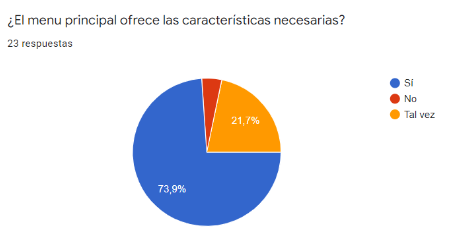
\includegraphics[width=0.9\textwidth]{Images/Capitulo8/Capitulo8.2/grafico3.png}
    \caption{Resultado de la pregunta de página principal intuitiva}
    \label{fig:grafico_3}
\end{figure}

%%%%%%%%%%%%%%%%%%%%%%%%%%%%%
En la figura \ref{fig:grafico_4} se puede observar que nadie piensa que el perfil no cuente con la información necesaria para lo que está destinada la aplicación.

\begin{figure}[H]
    \centering
    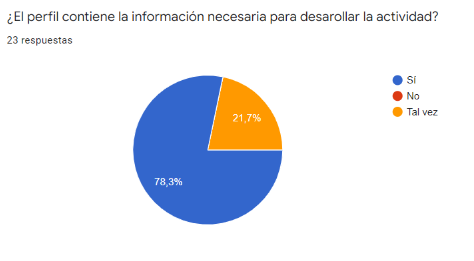
\includegraphics[width=0.9\textwidth]{Images/Capitulo8/Capitulo8.2/grafico4.png}
    \caption{Resultado de la pregunta de información en el perfil}
    \label{fig:grafico_4}
\end{figure}

%%%%%%%%%%%%%%%%%%%%%%%%%%%%%%
En la figura \ref{fig:grafico_5} se puede observar que un 65,2\% de los usuarios que han probado la aplicación no han creado una dieta frente a un 34,8\% de los usuarios si lo han hecho.

\begin{figure}[H]
    \centering
    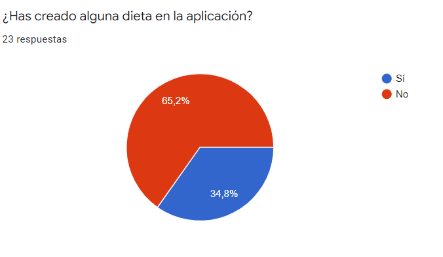
\includegraphics[width=0.9\textwidth]{Images/Capitulo8/Capitulo8.2/grafico5.png}
    \caption{Resultado de la pregunta de creación de dietas}
    \label{fig:grafico_5}
\end{figure}

%%%%%%%%%%%%%%%%%%%%%%%%%%%%%%%%

Como se puede observar en la figura \ref{fig:grafico_6} hay opiniones más diversas en cuanto a la complejidad de la creación de las dietas. Un 50\% les ha parecido fácil la creación de la dieta frente a un 37,5\% que les ha parecido compleja.

\begin{figure}[H]
    \centering
    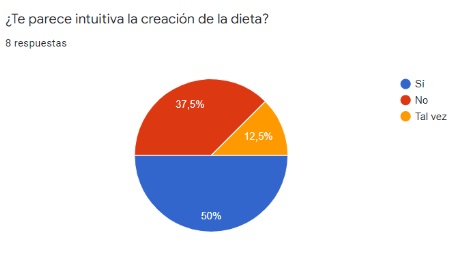
\includegraphics[width=0.9\textwidth]{Images/Capitulo8/Capitulo8.2/grafico6.png}
    \caption{Resultado de la pregunta del proceso de creación de una dieta}
    \label{fig:grafico_6}
\end{figure}

%%%%%%%%%%%%%%%%%%%%%%%%%%%%%%%%
En cuanto a la figura \ref{fig:grafico_7} se puede observar que solo un usuario respondió esta pregunta (se trata de una pregunta no obligatoria), opinando sobre una posible mejora respecto a la generación de una dieta.

\begin{figure}[H]
    \centering
    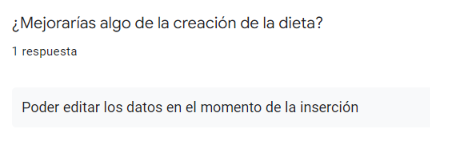
\includegraphics[width=0.9\textwidth]{Images/Capitulo8/Capitulo8.2/grafico7.png}
    \caption{Resultado de la pregunta de mejoras en la aplicación}
    \label{fig:grafico_7}
\end{figure}

%%%%%%%%%%%%%%%%%%%%%%%%%%%%%%%
Se puede observar en la figura  \ref{fig:grafico_8}  que un 73,9\% de los usuarios han seguido alguna dieta en el tiempo que estuvo probando la aplicación frente a un 26,1\% que no lo hizo.

\begin{figure}[H]
    \centering
    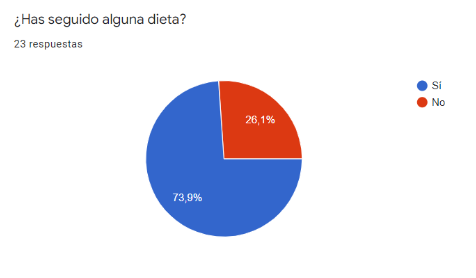
\includegraphics[width=0.9\textwidth]{Images/Capitulo8/Capitulo8.2/grafico8.png}
    \caption{Resultado de la pregunta de seguimiento de una dieta}
    \label{fig:grafico_8}
\end{figure}
%%%%%%%%%%%%%%%%%%%%%%%%%%%%%%

Se puede observar en la figura \ref{fig:grafico_9} que no ha habido ningún usuario que no le parezca intuitiva la inserción de alimentos.

\begin{figure}[H]
    \centering
    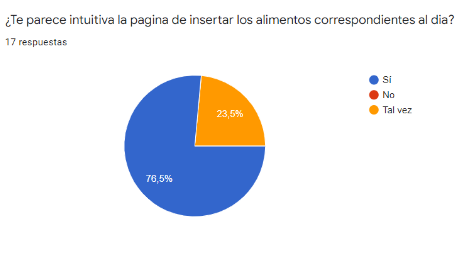
\includegraphics[width=0.9\textwidth]{Images/Capitulo8/Capitulo8.2/grafico9.png}
    \caption{Resultado de la pregunta de inserción de alimentos en una dieta}
    \label{fig:grafico_9}
\end{figure}
%%%%%%%%%%%%%%%%%%%%%%%%%%%%%%%%

En la figura \ref{fig:grafico_10} se puede observar que un 58,8\% de los usuarios encuentran utilidad a la sección de comentarios de la dieta frente a un 11,8\% que no lo encuentran.

\begin{figure}[H]
    \centering
    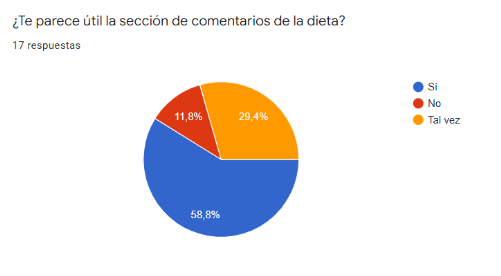
\includegraphics[width=0.9\textwidth]{Images/Capitulo8/Capitulo8.2/grafico10.png}
    \caption{Resultado de la pregunta de utilidad de los comentarios}
    \label{fig:grafico_10}
\end{figure}
%%%%%%%%%%%%%%%%%%%%%%%%%%%%%%%%%%

En la figura \ref{fig:grafico_11} se encuentra un comentario de una persona ofreciendo una posible mejora a la aplicación en la sección de seguimiento de la dieta.

\begin{figure}[H]
    \centering
    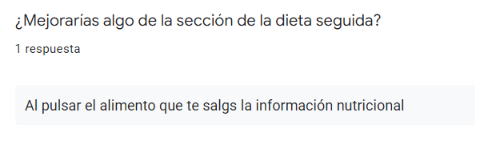
\includegraphics[width=0.9\textwidth]{Images/Capitulo8/Capitulo8.2/grafico11.png}
    \caption{Resultado de la pregunta de mejoras en seguimiento de la dieta}
    \label{fig:grafico_11}
\end{figure}
%%%%%%%%%%%%%%%%%%%%%%%%%%%%%
Como se puede observar en la figura \ref{fig:grafico_12} la valoración general de la aplicación tiene una media de 7,52  en unas 23 respuestas insertadas por los usuarios.

\begin{figure}[H]
    \centering
    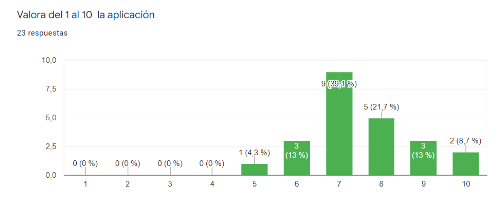
\includegraphics[width=0.9\textwidth]{Images/Capitulo8/Capitulo8.2/grafico12.png}
    \caption{Resultado de la pregunta de valoración general de la aplicación}
    \label{fig:grafico_12}
\end{figure}
%%%%%%%%%%%%%%%%%%%%%%%%%%%%%%%%%%%%

Respecto a la figura \ref{fig:grafico_13} se puede observar un comentario de una persona en la que valora una posible mejora para la aplicación.

\begin{figure}[H]
    \centering
    
\includegraphics[width=0.9\textwidth]{Images/Capitulo8/Capitulo8.2/grafico13.png}
    \caption{Resultado de la pregunta de funcionalidades extra}
    \label{fig:grafico_13}
\end{figure}